%\documentclass[xcolor=table,handout,compress]{beamer}
\documentclass[xcolor=table,aspectratio=169]{beamer}
%--------------------------------------------------------------------------
% Common packages
%--------------------------------------------------------------------------
\usepackage[english]{babel}
\usepackage{pgfpages} % required for notes on second screen
\usepackage{graphicx}
\usepackage{subfigure}
\usepackage{multicol}
\usepackage[normalem]{ulem}

\usepackage{tabularx,ragged2e}
\usepackage{booktabs}
\usepackage{marvosym}

\makeatletter
\let\beamer@writeslidentry@miniframeson=\beamer@writeslidentry
\def\beamer@writeslidentry@miniframesoff{%
  \expandafter\beamer@ifempty\expandafter{\beamer@framestartpage}{}% does not happen normally
  {%else
    % removed \addtocontents commands
    \clearpage\beamer@notesactions%
  }
}
\newcommand*{\miniframeson}{\let\beamer@writeslidentry=\beamer@writeslidentry@miniframeson}
\newcommand*{\miniframesoff}{\let\beamer@writeslidentry=\beamer@writeslidentry@miniframesoff}
\makeatother


%--------------------------------------------------------------------------
% Load theme
%--------------------------------------------------------------------------
\usetheme{hri}

\usepackage{tikz}
\usetikzlibrary{patterns,shapes,fpu,fit,calc,mindmap,backgrounds,positioning,svg.path}


\tikzset{
  invisible/.style={opacity=0},
  visible on/.style={alt={#1{}{invisible}}},
  alt/.code args={<#1>#2#3}{%
    \alt<#1>{\pgfkeysalso{#2}}{\pgfkeysalso{#3}} % \pgfkeysalso doesn't change the path
  },
}

\newcommand*\circled[1]{\tikz[baseline=(char.base)]{
            \node[shape=circle,draw,inner sep=1pt] (char) {\bf\tiny #1};}}


%% Neat trick to have only one navigation bullet per subsection
%% http://tex.stackexchange.com/questions/64333/one-navigation-bullet-per-subsection-with-subsection-false-in-custom-beamer-them
%\usepackage{etoolbox}
%\makeatletter
%\patchcmd{\slideentry}{\advance\beamer@xpos by1\relax}{}{}{}
%\def\beamer@subsectionentry#1#2#3#4#5{\advance\beamer@xpos by1\relax}%
%\makeatother
%%%%%%%%%%%%%%%%%%%%%%%%%%%%%%%%%%%%%%%

\graphicspath{{figs/}}

% for model of anthopomorphism
\newcommand{\IPA}{{$\mathcal{A}_0$~}}
\newcommand{\SLA}{{$\mathcal{A}_\infty$~}}
\newcommand{\sla}{{\mathcal{A}_\infty}}
\newcommand{\AntMax}{{$\mathcal{A}_{max}$~}}
\newcommand{\antMax}{{\mathcal{A}_{max}}}

% for HATP plans
\newcommand{\hatpaction}[3]{#1\\\textsf{\scriptsize #2,}\\\textsf{\scriptsize #3}}
\newcommand{\stmt}[1]{{\footnotesize \tt  #1}}

% for mutual modelling
\newcommand{\Mmodel}[3]{{\mathcal{M}(#1, #2, #3)}}
\newcommand{\model}[3]{{$\mathcal{M}(#1, #2, #3)$}}
\newcommand{\Model}[3]{{$\mathcal{M}^{\circ}(#1, #2, #3)$}}

% typeset logical concept
\newcommand{\concept}[1]{{\scriptsize \texttt{#1}}}

\newcommand{\backbutton}{\hfill\hyperlink{appendix}{\beamerreturnbutton{Supplementary material}}}
%--------------------------------------------------------------------------
% General presentation settings
%--------------------------------------------------------------------------
\title{\Large Understandability}
\subtitle{Some food for thought in the context of HRI}
\date{{\bf Responsible Robotics} | Dagstuhl Seminar, 11-15 Sep 2023}
\author{Séverin Lemaignan}
\institute{{\bf PAL Robotics} Head of Social Robotics, Senior Scientist AI \& HRI}

%--------------------------------------------------------------------------
% Notes settings
%--------------------------------------------------------------------------
%\setbeameroption{show notes on second screen}
%\setbeameroption{hide notes}

\begin{document}


%%%%%%%%%%%%%%%%%%%%%%%%%%%%%%%%%%%%%%%%%%%%%%%%%%%%%%%%


%%%%%%%%%%%%%%%%%%%%%%%%%%%%%%%%%%%%%%%%%%%%%%%%%%%%%%%%

\licenseframe{github.com/severin-lemaignan/2023-understandability-dagstuhl}

\maketitle
\imageframe{my_background/bg-map}



\begin{frame}<2-7>[label=soro]{Social Robotics}
    \centering

    \begin{columns}
        \begin{column}{0.7\linewidth}

            \only<1>{
                Creating interactive robots that are \textbf{embedded and
                understand their (human) social context}; \textbf{generate and adopt appropriate
                social behaviours}; have a \textbf{positive impact on human
                society}.

                \vspace{2em}
                $\Rightarrow$ designing and implementing the \textbf{assistant and
                companion robots} for  tomorrow.

                \vspace{2em}
                $\Rightarrow$ direct impact on ageing society, education, customer service;
                \textbf{major socio-economic
                challenge}

                \vspace{2em}
                $\Rightarrow$ but also: \textbf{unique opportunity to provide individualised
                support for vulnerable populations}
            }

            \only<2->{
                \textbf{Major scientific challenges}:

                \begin{itemize}
                    \item<2-> Model open-ended, underspecified situations; rich
                        semantics; complex social dynamics;
                    \item<3-> Close the interaction loop;
                    \item<4-> Understand and sustain long-term autonomous social interactions;
                    \item<5-> Real-world algorithmic robustness;
                    \item<6-> Complex ethical landscape;
                    \item<7-> $\Rightarrow$ cross-disciplinary \& holistic approach required
                    \item<7-> $\Rightarrow$ involve all the stakeholders;
                        participatory approach

                \end{itemize}


                \uncover<8>{
                \vspace{1em}


                \setbeamercolor{hriSec1Demo}{bg=hriSec3Dark,fg=white}
                \begin{beamercolorbox}[wd=\linewidth,ht=8ex,dp=0.7ex]{hriSec1Demo}
                    \large \bf \centering
                    Socially-Driven Autonomous Robots \\
                    for \\
                    Real-world Human-Robot Interactions
                \end{beamercolorbox}
            }


            }
        \end{column}
        \begin{column}{0.35\linewidth}
            \begin{center}
                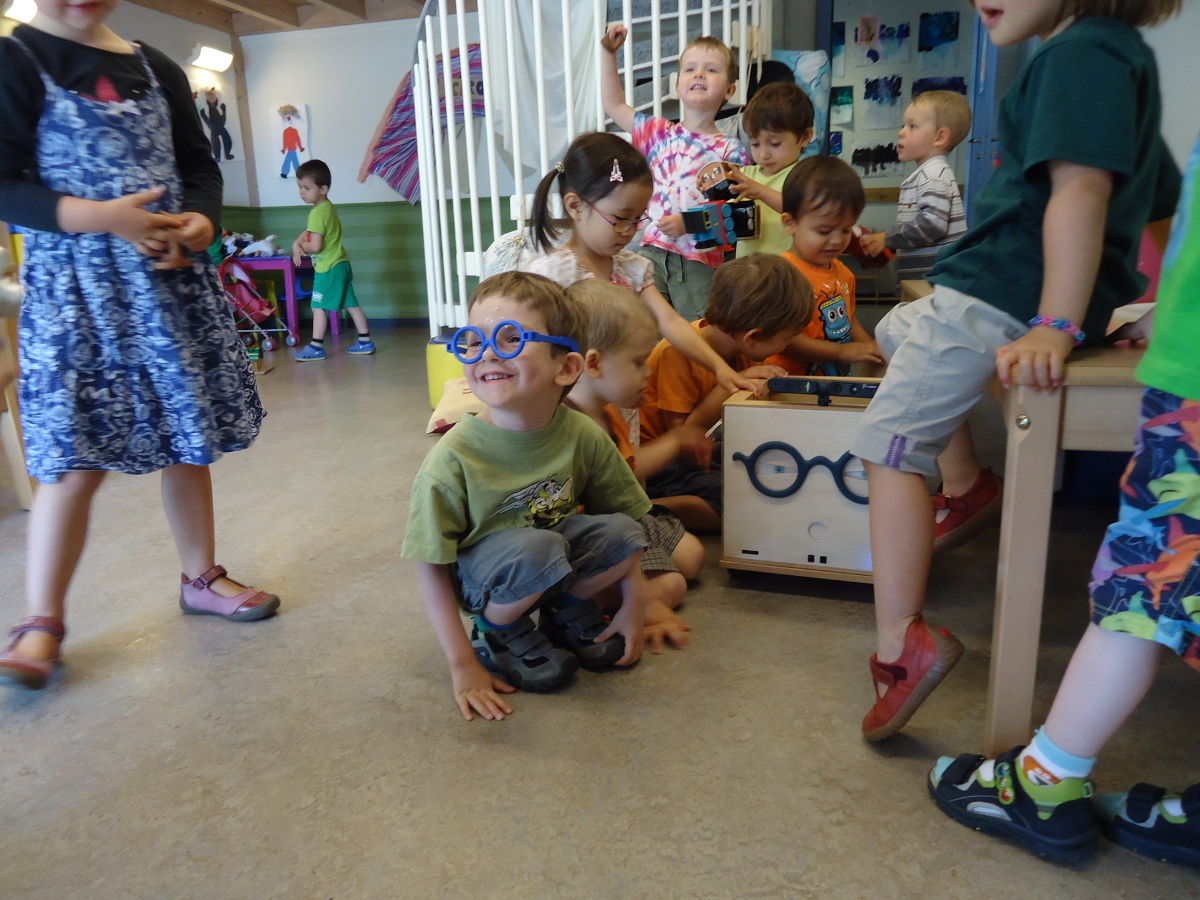
\includegraphics[trim=15cm 0 11cm 0,clip,width=0.7\linewidth]{ranger/ranger_funny_glasses}
            \end{center}
        \end{column}
    \end{columns}

    \toplogo{logo_bw}
\end{frame}

\section*{Understandability}

\begin{frame}{Understandability}

    ...`Understandability'?

    \pause

    In EU's \href{https://digital-strategy.ec.europa.eu/en/library/ethics-guidelines-trustworthy-ai}{Ethics Guidelines
    for Trustworthy AI}, keywords like:

    \begin{itemize}
        \item transparency
        \item explainability (eg XAI)
        \item tracability (eg Winfield's \emph{ethical black box})
    \end{itemize}

    \pause

    Useful mechanistic approach, ...but does it capture well the \emph{feeling}
    of `understanding' the machine? (ie, in-situ, in-the-moment, intuitive
    understanding)

    \pause

    In other words, would eg explainability and tracability by themselves be
    sufficient to establish trust?

    \toplogo{logo_bw}
\end{frame}

\begin{frame}{Do we actually really want to understand our robots?}

    Users (ourselves included) want technology that `just work'; cf Obadia's idea of the inherent \emph{magic} of technology

    \pause

    Example: when people ask something to ChatGPT, they might complain that the
    result is incorrect (hallucinated or otherwise) $\Rightarrow$ they
    want the visible, \emph{surface} result to fixed.

    \pause

    Do they want to \emph{understand} why ChatGPT got it wrong? I'd argue that
    the vast majority do not really care.

    \pause

    However, I would also argue that, to trust the system, what we really want
    is to be able to \alert<5>{confidently}\bubblemark{mark1} build a
    \alert<6>{robust mental model}\bubblemark{mark2}, with a strong \bubblemark{mark3}\alert<7>{predictive
    power}.

%    \bubble<5>[200][0.5][6cm]{mark1}{extrapolating from known mental models;
%    building the model implicitly while interacting;...}
%    \bubble<6>[220][0.5][5cm]{mark2}{once established, the model remains
%    essentially stable and
%    valid over time}
%    \bubble<7>[300][0.5][5cm]{mark3}{this foster the resulting trust}

    \toplogo{logo_bw}
\end{frame}

{
\paper{Lemaignan, Fink, Dillenbourg, Braboszcz {\bf The Cognitive Correlates of Anthropomorphism}, HRI 2014}
\begin{frame}{Cognitive Interpretation?}

    \vspace{-1em}
    \begin{figure}
        \centering
        \resizebox{0.9\paperwidth}{!}{
            \begin{tikzpicture}
                \baselineskip=8pt

                \path[fill=hriSec1Comp!50] (0,0) rectangle (10.5,2);
                \path[fill=hriSec1!50] (0,2) rectangle (10.5,4);
                \path[fill=hriSec3Comp!50] (0,4) rectangle (10.5,6);

                \draw (-0.3,1) node[rotate=90] {Stage 1}
                (-0.3,3) node[rotate=90] {Stage 2}
                (-0.3,5) node[rotate=90] {Stage 3};

                \draw[->] (0,0) -- (11,0) node[anchor=north] {$t$};
                \draw[-|] (0,0) -- (0,6.5) node[anchor=east] {};
                % Us
                \draw[ultra thick, ->] (0,0) -- (1,2) -- (3,2) -- (4,4) -- (6,4) -- (7,6) --
                (9.5,6);
                \draw[ultra thick, dashed, ->] (3,2) -- (9.5,2);
                \draw[ultra thick, dashed, ->] (6,4) -- (9.5,4);

                \draw (11,1) node[align=left, anchor=west]{\scriptsize pre-cognitive\\\scriptsize anthropomorphism}; %label

                \draw (11,3) node[align=left, anchor=west] {\scriptsize{projection of existing}\\\scriptsize{mental models}\\\scriptsize{\it (familiarity)}}; %label

                \draw (11,5) node[align=left, anchor=west] {\scriptsize{adapted mental
                model} \\ $\to$ \scriptsize{adapted interaction}\\\scriptsize{\it (anthropomorphic or not)}}; %label


                \draw[dashed,->] (1,0.1) to[bend right] (2,1.9)  node at (4.5,1) {\tiny{\it observation (shape, motion, sound)}}; %label

                \draw[dashed,->] (4,2.1) to[bend right] (5,3.9)  node[align=left] at (7.5,3) {\tiny \it observation (interactive behavior) \\ \tiny \it or short interaction}; %label

                \draw[dashed,->] (7,4.1) to[bend right] (8,5.9)  node[align=left] at (9,5)
                {\tiny \it contextualized\\ \tiny \it interaction}; %label

            \end{tikzpicture}
        }
    \end{figure}

    \badge[caption=Julia Fink]{colleagues/julia}
    %\toplogo{logo_bw}
\end{frame}
}

\begin{frame}{What means `responsible' in that context?}
    If we adopt the cognitive perspective of \emph{understanding} the robot as
    the \textbf{completion of a robust mental model} of the machine, where does
    that leave us wrt. \emph{responsible} understandability?

    \pause

    $\Rightarrow$ design robots' behaviours to foster the creation of detailed
    and correct mental models

    \pause

    ...or even let the end-users co-design the robot's cognitive capabilities

    \toplogo{logo_bw}
\end{frame}

\section*{`End-to-end' co-design}

\imageframe[color=black,caption=End-to-end co-design: gym coach]{couch25k/hri-169.jpg}

{
    \paper{Winkle et al. \textbf{In-Situ Learning from a Domain Expert for Real World Socially Assistive Robot Deployment} RSS 2020}

\begin{frame}{Couch-to-5k study}

    \vspace{0.2cm}

    \begin{columns}
        \begin{column}{0.5\linewidth}
                \centering
                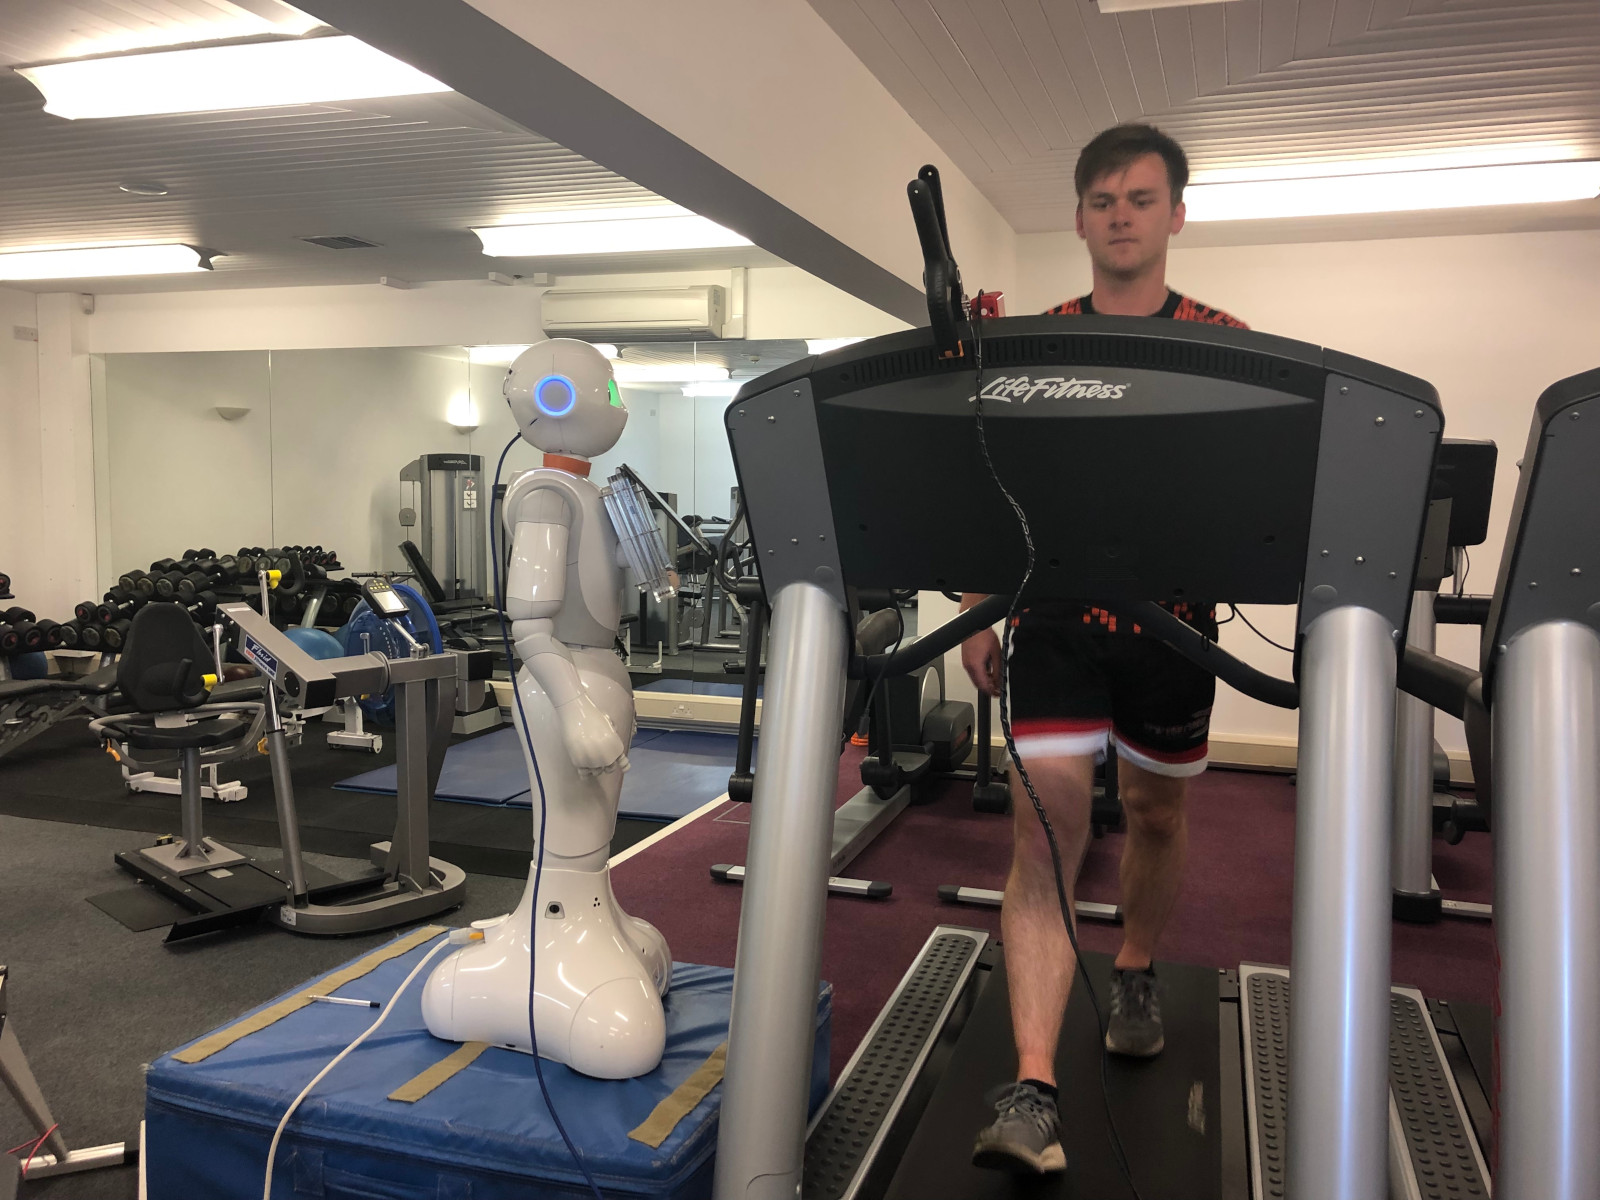
\includegraphics[height=3cm]{couch25k/hri.jpg}
        \end{column}
        \begin{column}{0.5\linewidth}
                \centering
                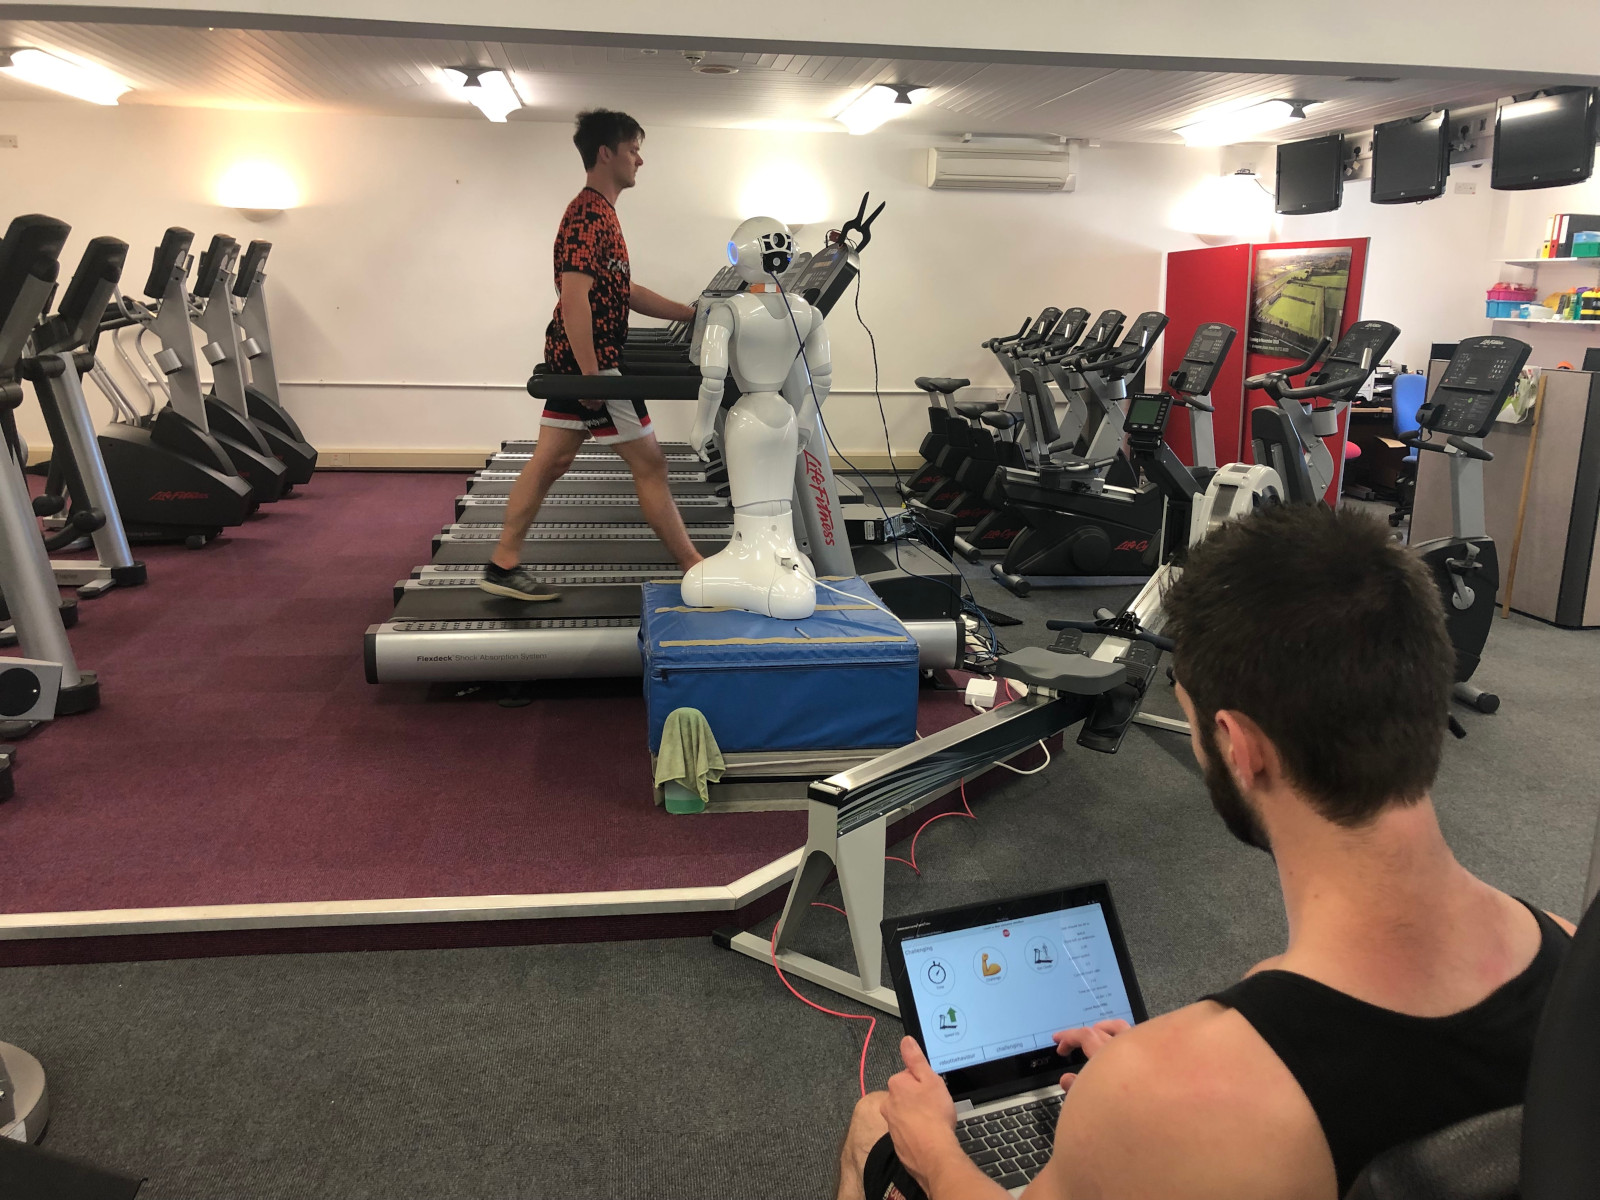
\includegraphics[height=3cm]{couch25k/supervised.jpg}
        \end{column}
    \end{columns}

    \begin{itemize}
        \item 9 participants
        \item 3 months; 27 one-hour sessions per participants
        \item $|state| = 20$; $|action\_space| = 11$
        \item Includes participants' personality (Big-5) as input feature
    \end{itemize}

    %\toplogo{logo_bw}
    \badge[caption=Katie Winkle]{colleagues/katie}
\end{frame}
}

{
    \paper{Winkle et al. \textbf{In-Situ Learning from a Domain Expert for Real World Socially Assistive Robot Deployment} RSS 2020}

\begin{frame}{Co-design for real-world + long-term}

    \begin{center}
        \resizebox{!}{0.75\pageheight}{
        \begin{tikzpicture}
            \node at (0,0) {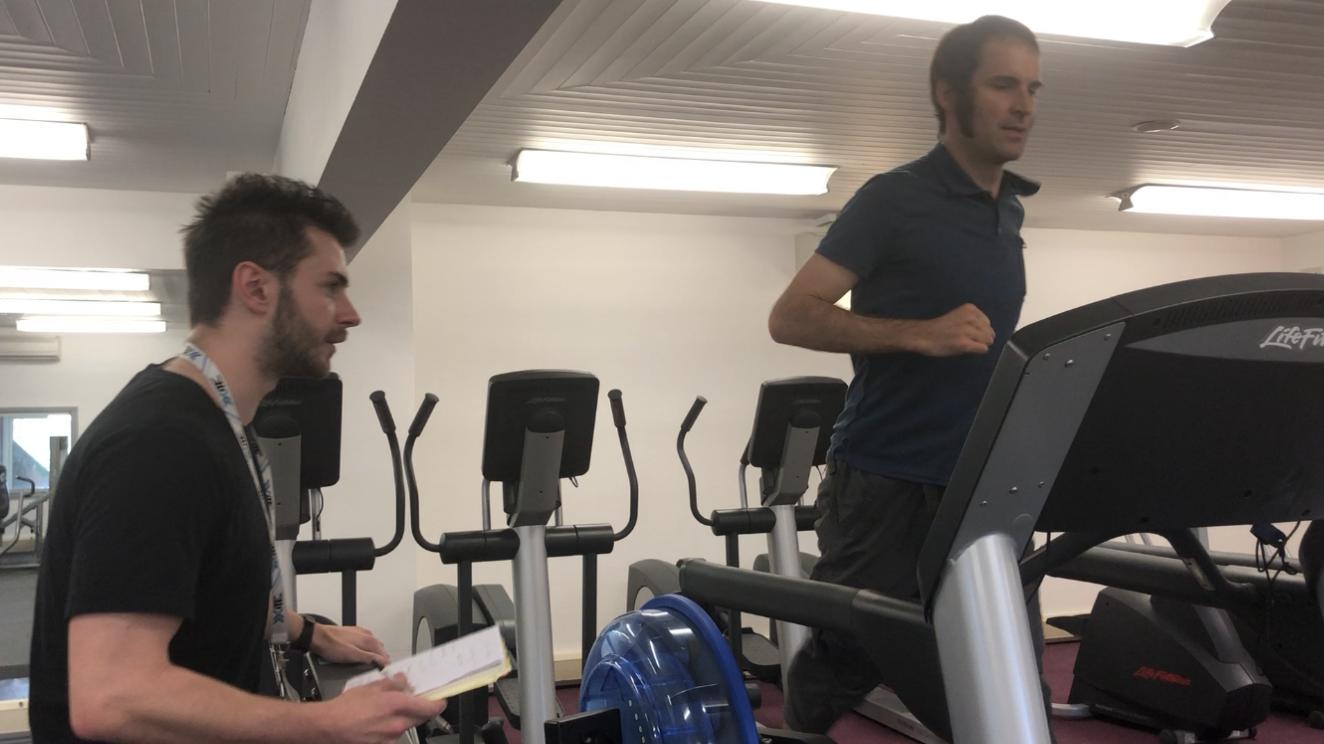
\includegraphics[width=0.6\linewidth]{figs/couch25k/couch25km-mock.jpg}};
           \node[anchor=north] at (7,0.5) {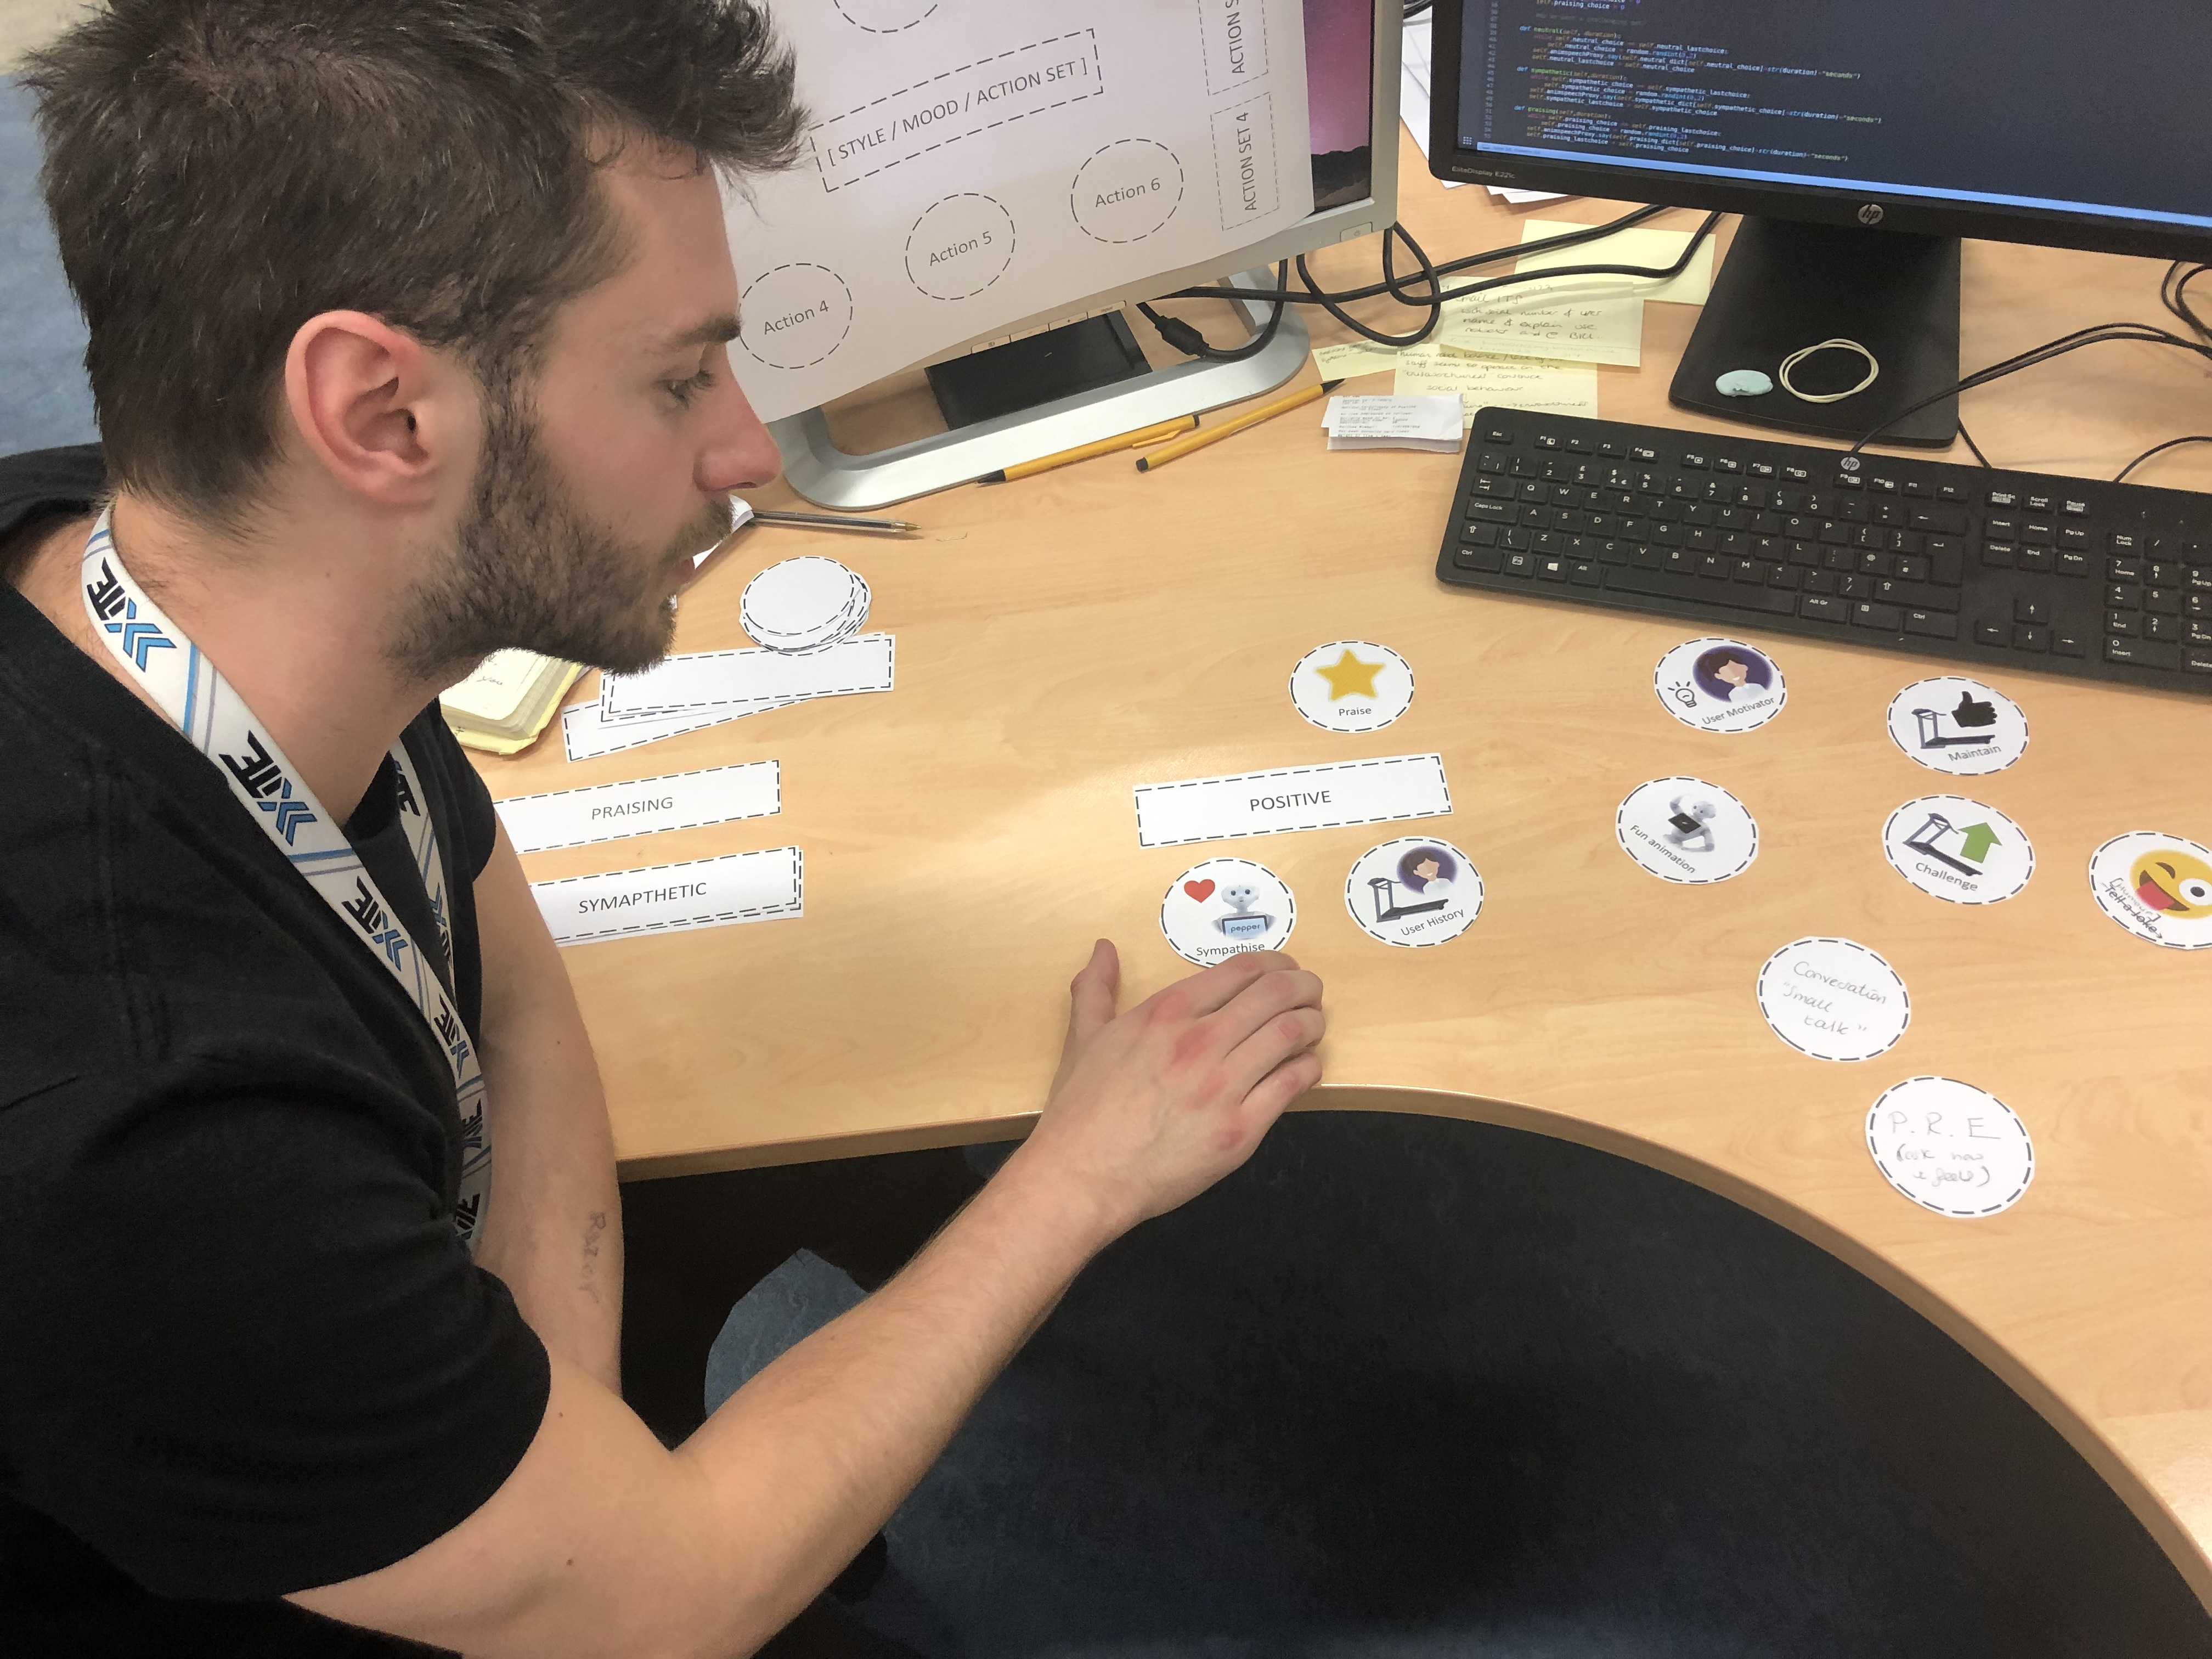
\includegraphics[trim=0 15cm 0 0,clip,width=0.6\linewidth]{figs/couch25k/codesign.jpg}};
           \node[anchor=north] at (-3.5,-1.5) {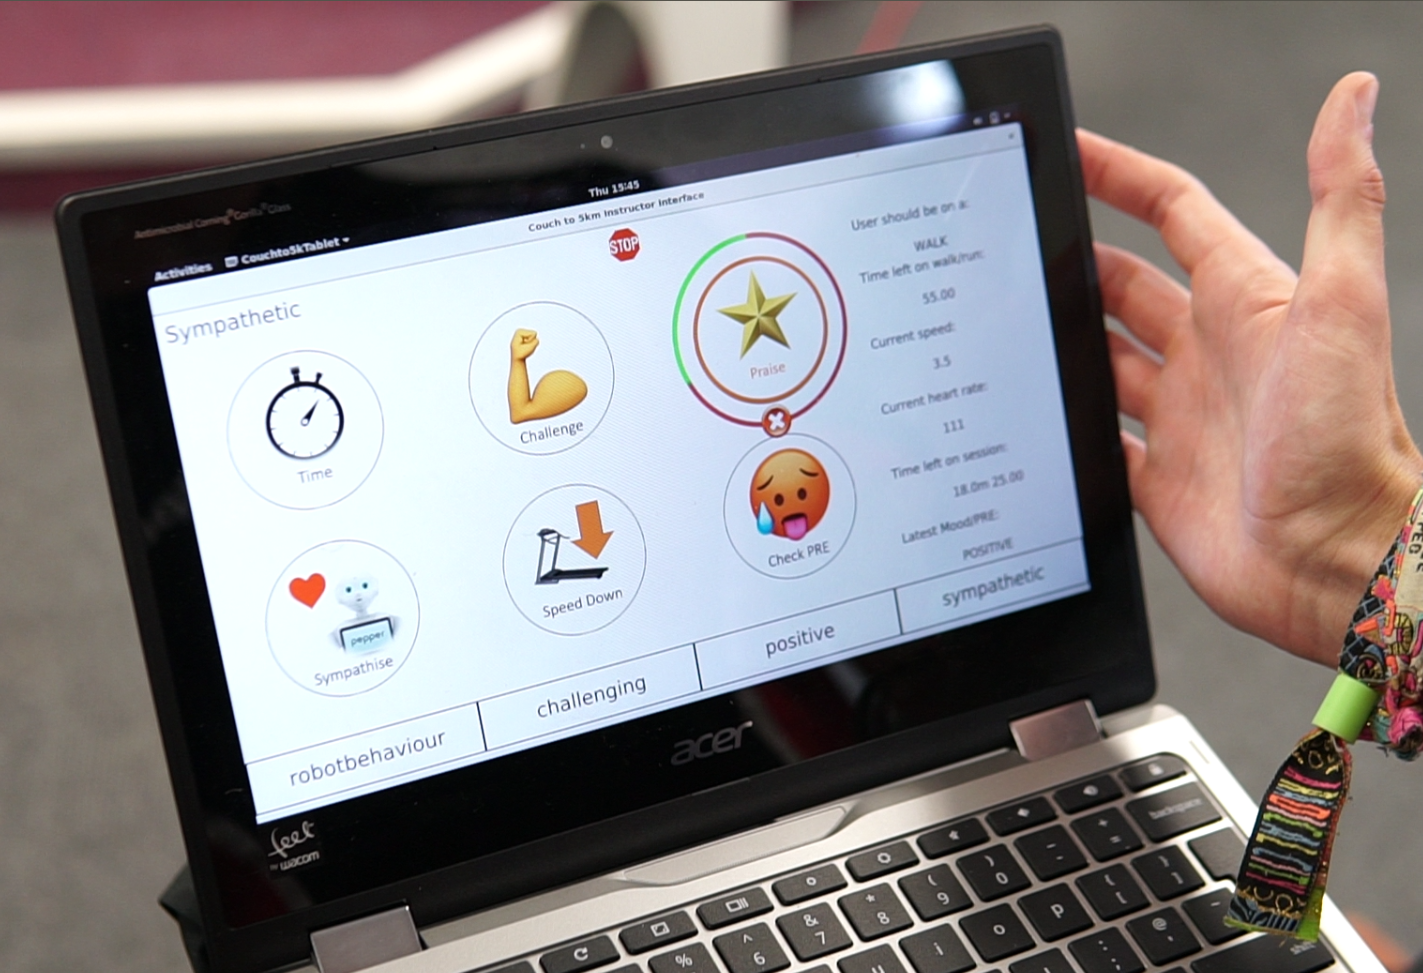
\includegraphics[width=0.5\linewidth]{figs/couch25k/teacher-ui.png}};
        \end{tikzpicture}
    }

    \end{center}
    %\toplogo{logo_bw}
    \badge[caption=Katie Winkle]{colleagues/katie}
\end{frame}
}


\imageframe[scale=0.9]{DesignProcess-base}
\imageframe[scale=0.9]{DesignProcess-irl}
\imageframe[scale=0.9]{DesignProcess-full}



{
    \paper{Winkle et al. \textbf{In-Situ Learning from a Domain Expert for Real World Socially Assistive Robot Deployment}
    RSS 2020}
    \begin{frame}{Learnt policies}
        \begin{center}
            \includegraphics<1>[width=0.9\linewidth]{figs/couch25k/finalactiondist-no-autonomous.png}
            \includegraphics<2>[width=0.9\linewidth]{figs/couch25k/finalactiondist.png}
            \includegraphics<3>[width=0.9\linewidth]{figs/couch25k/fullcomp_lbmr.pdf}
        \end{center}
    \toplogo{logo_bw}
\end{frame}
}


{
    \paper{Senft et al. \textbf{SPARC: Supervised progressively autonomous
robot competencies}, ICSR 2015;\newline
    Winkle et al. \textbf{LEADOR: End-to-End Participatory
    Design of Autonomous Social Robots} FrontiersIn AI \& Robotics 2021}
\begin{frame}{LEADOR: end-to-end co-design}

    \begin{columns}
        \begin{column}{0.6\linewidth}
    \begin{itemize}
        \item a successful technical solution to replace the wizard;
        \item but equally important, a \textbf{end-to-end} participatory design
            methodology (\emph{LEADOR: Led-by-Experts Automation \\and Design Of
            Robots})
    \end{itemize}



        \end{column}
        \begin{column}{0.4\linewidth}
            \begin{center}

               % \includegraphics<1>[width=\columnwidth]{DesignProcess-base}
               % \includegraphics<2>[width=\columnwidth]{DesignProcess-irl}
                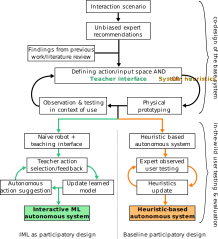
\includegraphics[width=\columnwidth]{DesignProcess-full}
            \end{center}
        \end{column}
    \end{columns}

    %\toplogo{logo_bw}
    \badge[caption=Emmanuel + Katie]{colleagues/emmanuel_katie}
\end{frame}
}

\begin{frame}{}

    More importantly,

    \vspace{2em}

    \begin{center}

    \large{``It was like training my assistant. Now I let it start with the
    next participant, while I do stretching with the previous one.''}

    \end{center}

    \vspace{2em}

    \pause

    ...does he \emph{understand} the robot? \footnotesize{yes and no}

    \pause

    \normalsize ...is it \emph{Responsible Robotics\textcopyright}?

    \toplogo{logo_bw}
\end{frame}


\section*{Very brief look at the industry}

\begin{frame}{Does it translate to industry?}
    \begin{columns}
        \begin{column}{0.7\linewidth}
            \only<1-2>{
            Can we turn the LEADOR paradigm into a generic \& robust enough technique for broad usage?
            }

            \only<2>{
                \vspace{1cm}
                \textbf{Two key use-cases for PAL Robotics}:

            \begin{itemize}
                \item robots that know when to help in public administrations
                \item elderly care and isolation (but... \textbf{rHHI}:
                    robot-supported Human-Human Interactions!)
            \end{itemize}
            }

        \end{column}
        \begin{column}{0.3\linewidth}
            \begin{center}
                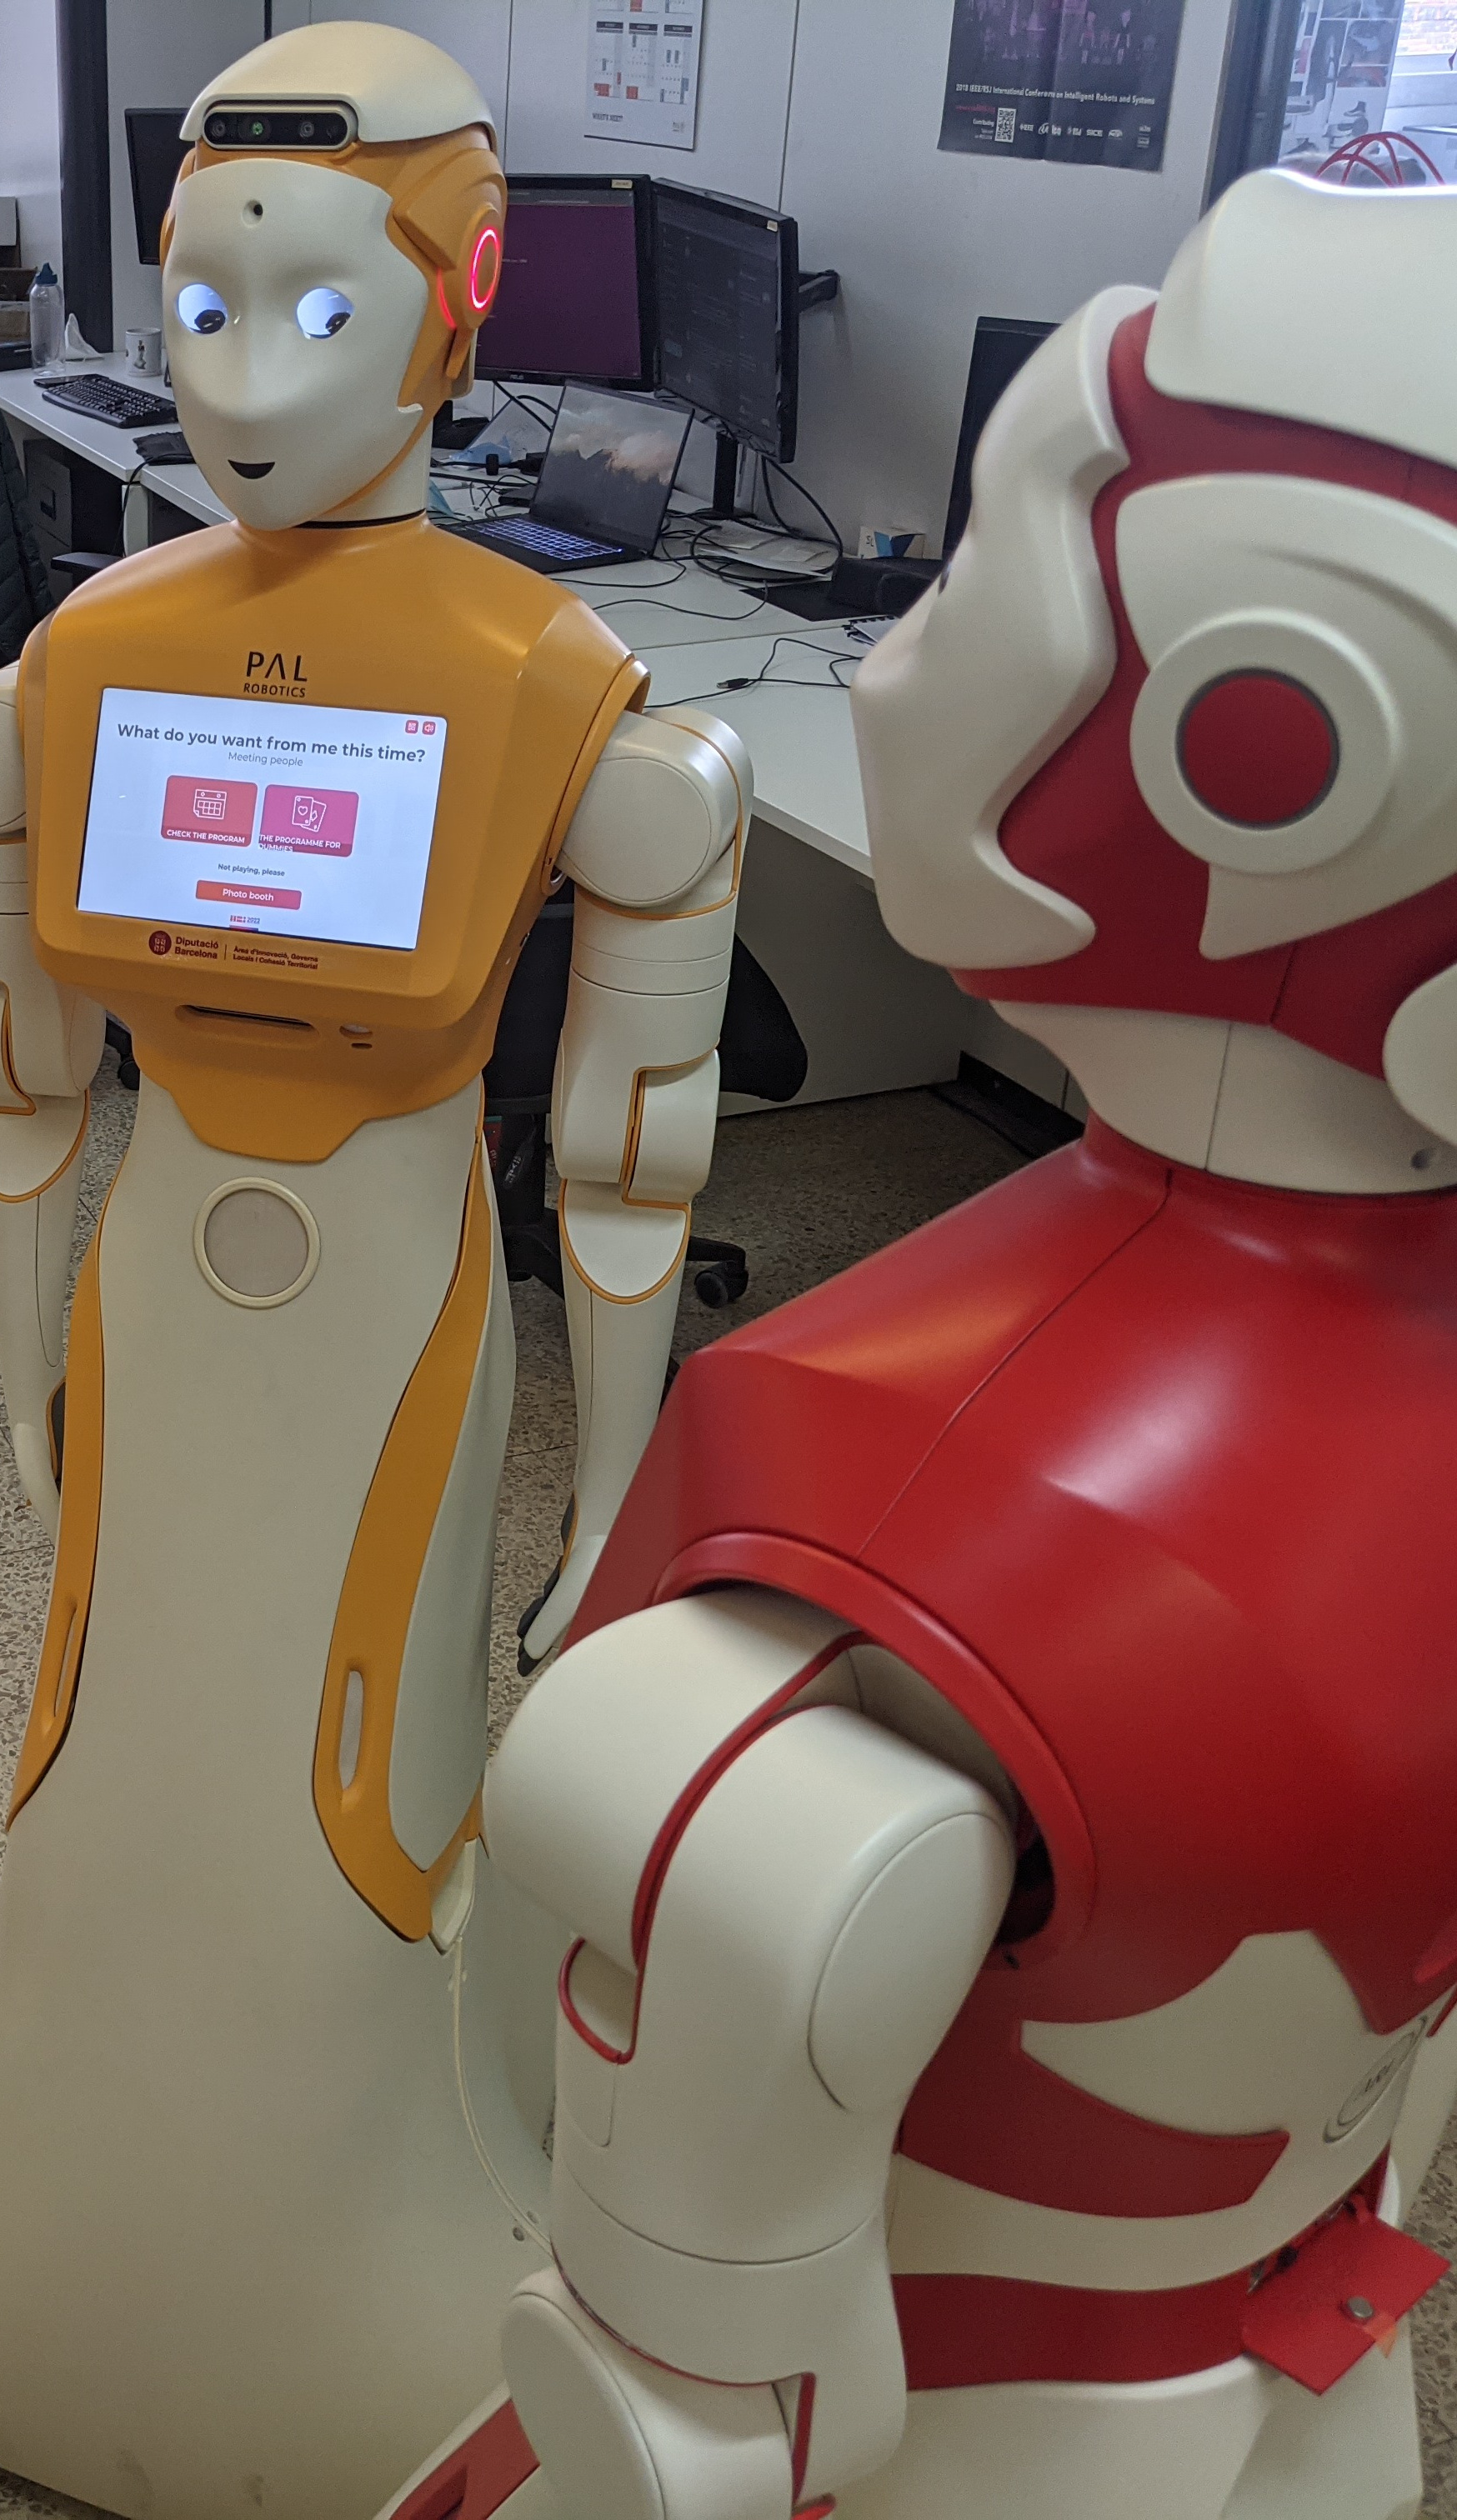
\includegraphics[height=0.7\pageheight]{figs/aris.jpg}
            \end{center}
        \end{column}
    \end{columns}

    \toplogo{logo_bw}

\end{frame}

\imageframe[caption=NHoA: Never HOme Alone]{nhoa/miro-interviews}
\imageframe[caption=H2020 SHAPES]{shapes/visitsmallorca}
\imageframe[color=black, caption=AMIBA]{amiba/amiba-1}
\imageframe[color=black, caption=AMIBA]{amiba/amiba-2}
\imageframe[color=black, caption=AMIBA]{amiba/amiba-3}

\begin{frame}{Does it translate to industry?}
    \begin{columns}
        \begin{column}{0.7\linewidth}
            \begin{itemize}
                \item<+-> practical issues are typically overlooked (co-design
                    in-situ)
                 \item<+-> adoption: primarily from \emph{secondary} users (carers,
                    teachers...)
                \item<+-> needs are not always what we think (co-design with all
                    stakeholders)
                \item<+-> robots do not live in isolation: think 'eco-systems'
                    and embrace ``mis-use"/mis-understanding of the robot
                \item<+-> from interaction to habits: (individualised) long-term
                    \emph{mutual shaping}
                \item<+-> importance of the regulatory framework (legal +
                    ethical) to steer an
                    otherwise `engineering-focused' mindset

            \end{itemize}
        \end{column}
        \begin{column}{0.3\linewidth}
            \begin{center}
                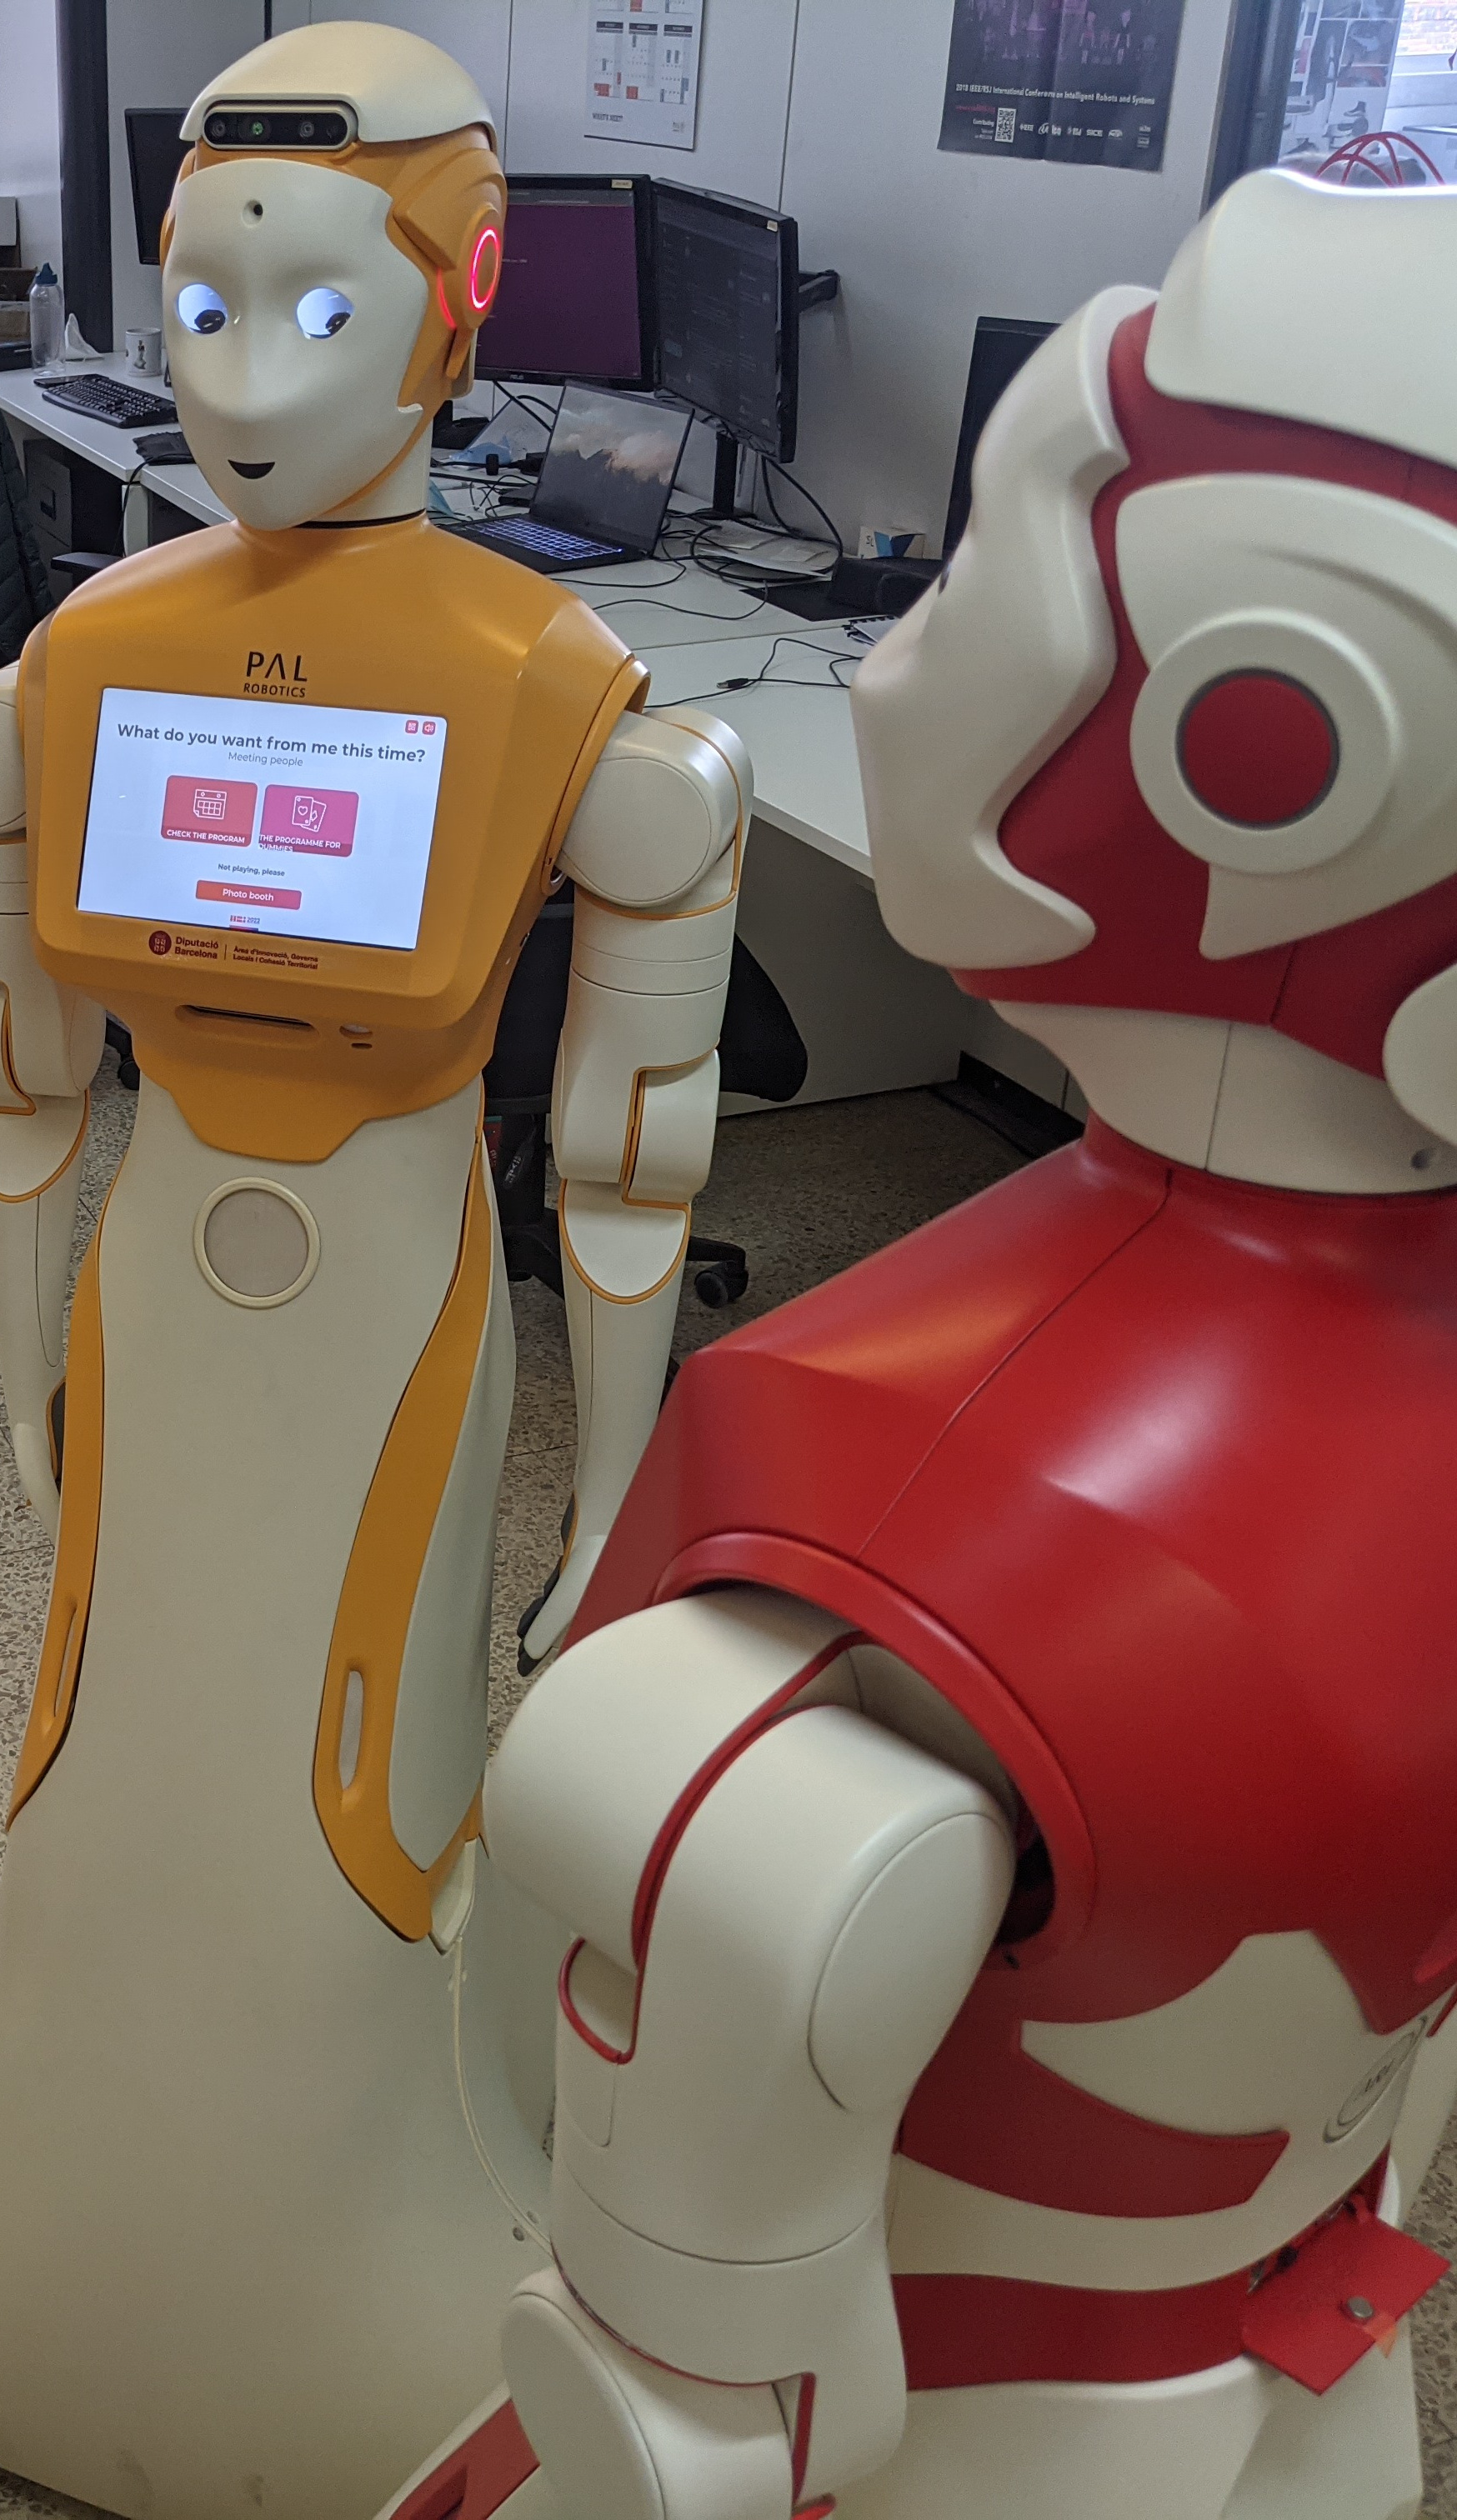
\includegraphics[height=0.7\pageheight]{figs/aris.jpg}
            \end{center}
        \end{column}
    \end{columns}

    \toplogo{logo_bw}

\end{frame}

\section*{Final remarks}

\begin{frame}{Some final remarks}

    \only<1>{
        Co-design requires bootstrapping: you need to understand at
            \emph{some} level the physical (easy) and cognitive (much harder)
            capabilities of the robot to `invent' its role

            $\rightarrow$ iterative process

            $\rightarrow$ slow process

            \footnotesize{(though more of a problem for traditional co-design than lifelong,
            end-to-end co-design)}

        }

    \only<2>{
    Sabanovic's \emph{mutual shaping} is fundamental and not yet fully
    internalised by researchers/engineers

    $\rightarrow$ you (re)shape your relation to -- and understanding of -- the robot by using it

    $\Rightarrow$ \emph{Understanding} the
    robot likely means that the robot also has to understand you!

    \footnotesize{(here, the meaning of \emph{understand} is left as an exercice
    to the reader)}
    }

    \only<3>{
        ...as such:

        can we really separate the human's understanding of the robot, from
        the robot's understanding of the human, of its environment, and... of
        itself? (introspection)
    }
\end{frame}

\begin{frame}{Anecdote: What if we ask the system to explain its behaviour?}

    \only<1-2>{
    \texttt{Sally (a girl) has 3 brothers. Each brother has 2 sisters. How many
    sisters does Sally have?}

    \pause

    GPT-4:

    \texttt{Sally has 2 sisters.}
}

    \only<3-4>{

    \texttt{Sally (a girl) has 3 brothers. Each brother has 2 sisters. How many
    sisters does Sally have?} \textbf{\texttt{Let's think step by step.}}

    \onslide<4>{

    GPT-4:

    \texttt{Sally has 3 brothers. Each of these brothers has 2 sisters. This means that there are 2 girls in the family, including Sally. Therefore, Sally has 1 sister.}

    (incidentally, \href{https://benchmarks.llmonitor.com/}{GPT-4 is the only model out of 60 tested that get the
    correct answer})
}
    }
 \toplogo{logo_bw}
\end{frame}


%%%%%%%%%%%%%%%%%%%%%%%%%%%%%%%%%%%%%%%%%%%%%%%%%%%%%%%%
{
    \fullbackground[color=black]{thank_you}
    \begin{frame}[plain]
    \end{frame}
}

\end{document}
